\documentclass[12pt, letterpaper]{article}
\setcounter{tocdepth}{2}
\usepackage[utf8]{inputenc}
\usepackage{hyperref}
\usepackage{xcolor}
\hypersetup{
colorlinks = true,
linkcolor = {black},
urlcolor = {blue},
}
\usepackage{epsfig, url}
\usepackage{epstopdf}
\usepackage{graphicx}
\usepackage{datetime}
\usepackage{multirow}

%\usepackage{wrapfig}
%\usepackage{amsmath}
\usepackage{amssymb}
\usepackage{geometry} 
\geometry{a4paper}              

\usepackage{titling}
\usepackage{tabto}
\usepackage{pdfpages}
\usepackage{hyperref}
\setlength{\evensidemargin}{0in}
\setlength{\oddsidemargin}{0in}
\setlength{\textwidth}{6.5in}
\setlength{\textheight}{9.0in}
\setlength{\topmargin}{0in}
\setlength{\headheight}{0in}
\setlength{\headsep}{0in}
\setlength{\itemsep}{-\parsep}



\begin{document}
\title{\large People Oriented Computing Assignment 2\\[0.5cm]
        \bf\Large Filming, Editing and Posting a video on TikTok}
\author{\large Mert Erol, 20-915-245}
\date{November 23rd, 2021}
\makeatletter
    \begin{titlepage}
        \begin{center}
        \vbox{}\vspace{5cm}
            {\@title }\\[3cm] 
            {\@author}\\
            %{Instructor: \bf instructor name}\\
            \vfill 
\includegraphics[scale=0.3]{images/logo.png}\\[1cm]
            {\@date}
        \end{center}
    \end{titlepage}
\makeatother
%\thispagestyle{empty}


\newpage
\tableofcontents
\newpage
%\listoftables
%\listoffigures
%\newpage


\section{Introduction}
For this assignment, the scenario is: "Filming, Editing and Posting a video on TikTok". We will evaluate this scenario using the "Abby" Persona from GenderMag and run two independent walk-throughs of this scenario using that persona. The first walk-through will be done by Mert Erol (20-915-245), from now on referred to as "Walk-through 1", while the second one was kindly provided by Luc Aggett (20-918-371), hence forth referred to as "Walk-through 2".\newline
Because using TikTok is not something that people with certain backgrounds have an advantage at, we did not think that it would make sense to make drastic changes to Abby's persona sheet. Therefore, the changes that have been made are rather small and simple. The above-mentioned walk-throughs and the Abby persona sheet will be attached at the end of this document.\\

\subsection{Scenario}
\begin{center}
    \begin{tabular}{|c|c|}
    \hline
        \textbf{Sub-goals} & \textbf{Actions} \\
        \\
        1. Film the video & 1. Open the App \\
        & 2. Press the button in the middle at the bottom \\
        & 3. Start filming by pressing the red button \\ 
        \\
        2. Edit the video & 1. Click on one of the submenus on the bottom left \\
        & 2. Look through each item in each submenu \\
        & 3. Chose the items you like in said submenu \\
        & 4. Repeat actions 1-3 with each submenu \\
        \\
        3. Post the video & 1. Press next on the bottom right \\
        & 2. Press on "describe your video" \\
        & 3. Enter a fitting caption \\
        & 4. Press on hashtags \\
        & 5. Enter fitting hashtags \\
        & 6.Decide on each of the clickables \\
        & 7. Press on post \\
        & 8. Press on post now \\
    \hline
    \end{tabular}
\end{center}
\newpage

\section{Analysis of the GenderMag Walk-throughs}
After completing both of the walk-throughs, it was clear that there were some problems, differences, and, of course, common grounds in our runs. In the following, we will further analyze some important points that are problematic and might help create small improvements by fixing those that, after a while, add up to a big improvement.\\
The subgoals and actions will be referred to by their assigned numbers as in the table above.

\subsection{Potentially Problematic Actions and Sub-goals}
If we only look at the sub-goals, there should not be any bigger problems that would make a huge difference to the outcome of the walk-through. What might create an issue for Abby in these first steps of realizing the sub-goals might be sub-goal number two, where the goal is to edit the video. This might pose a problem in that she is not familiar with editing videos. But on the other hand, for sub-goal one or three, there should not be any issues. In our opinion, using the facets we chose for Abby, we think that she should be able to come up with these sub-goals rather effortlessly.
Where some of the bigger problems might occur is in the actions needed to complete each one of the sub-goals. For example, in 1.2, Abby might not immediately realize how to open the recording submenu as she might not know what the symbol means on the screen as there is no explanation. In actions like 3.2, 3.4, and 3.6, where she needs to get creative and try out different hashtags (in the case of 3.4) etc., there might be some issues as well, as it involves some form of tinkering to really get the best out of this feature, but this will be explained in a further section.

\subsection{Relationship Between Problematic Aspects of the Interaction and The Facets}
We would like to start with sub-goal number 2. The problem that might occur here is mostly connected to the facet "Computer Self Efficacy" and the facet "Learning: by Process vs. by Tinkering". For this case, as Abby is not familiar with the TikTok app, she might not realize that she has to tinker or be ready to tinker inside the app to find the built-in editing submenu, and therefore she might choose to edit in a program she knows already or not edit at all.\\
The next points, namely 3.2, 3.4 and 3.6, can be grouped into one as the basic idea is pretty much the same. The user needs to be creative and tinker around to find the perfect hashtags (3.4), description (3.2) and properties of the video (3.6). This might pose the biggest challenge to Abby as the persona that has been used is created in such a way where Abby tries to tinkering and any risks while using unfamiliar technologies and instead gets her answers by looking up tutorials or just simply using technologies that she is already familiar with to achieve her goal.\newpage

\subsection{Problematic and/or Successful Features or Aspects of the System’s Design}
The largest problem we identified in the design of the system is that, depending on the used system, some actions are different or not even available. This we discovered in many steps of sub-goal 3 in this scenario. \\
In 3.4 where the action is "Press on Hashtags" this menu was not visible by the device used in walk-through 2. This problem lead to step 3.5 not being possible to be processed as this could not be fulfilled in this case.
A second large difference was seen in 3.7, where after pressing "Post", there was no second confirmation screen in walk-through 2 that prompted the user to make sure that they wanted to post this (3.8), contrary to walk-through 1, where this pop-up was visible. Problems such as the latter will not help with user friendliness because if you realize that you made a small mistake during sub-goal 2 and the actions in sub-goal 3 before the step of posting the video (3.7 and 3.8), you cannot go back and change it. You would have to delete the video completely and re-upload it by re-doing all the steps in sub-goals 2 and 3.\\
While this is one of the biggest issues we encountered with the aspects of the system's design, we can still say that the process of posting a video has great features as well that help the user greatly, and we would like to briefly discuss these features.\\
Now a point which might lead to some confusion as it does not make much sense when thinking about it. When the user downloads and uses the app for the first time, the app prompts the user to get a tour of the app and understand how the app works, but oddly enough, not in every facet or functionality of the app, which will be further discussed in the next section. This also happens when the user wants to create a video for the first time. With this simple but powerful feature, many users that are, in the case of this scenario, not that confident with using new technology or not ready to tinker with software are getting a great form of help without having to search or look up information on different platforms they are already familiar with. Another great feature is that, generally, most of the available features during content creation are mostly clearly labeled to help with ease-of-use and make the app as comfortable for everyone as possible.\newpage

\subsection{Other Problematic Aspects of the Interaction or Design Not Related to the Facets}
There are some points in the app's design that we realized might be bothersome for people using it for the first time or just starting to use it. To briefly list some aspects we want to mention in this section: When you open the app, videos start immediately playing and finding certain submenus that might prove useful, like where are the people I follow or follow me? How do I swap between submenus inside the app? How do I navigate inside the app? For someone who uses the app for the first time, all these questions will come up eventually. If not all, the least that will come up is the navigation inside the app, as nothing is explained regarding that point. \\
As soon as the user starts the app, the first problematic aspect catches the eye: videos immediately start playing. This might get very confusing for new users, as they might not know how to stop the video, and because of that, they are forced to close the app or fully lower the volume. Secondly, the submenus inside the app are not labeled for every device. This forces the user to tinker around and find everything on their own. This might be a big hassle for users who have to avoid tinkering at any cost, as they have to look up how to do the steps on web pages they know or ask friends. This last problem is, in our eyes, the biggest one of the three mentioned above, which is the navigation inside the app. Because the navigation is not really an intuitive one, it might be hard for users who get thrown into the deep end.

\subsection{Overall Assessment}
Content-creation apps like TikTok, where the user could be in any social and/or age group, are designed in such a way that everyone can understand and follow the steps to create, share, and also promote their own content once you get used to the app's design, although some issues are still present. Going through each sub-goal and each of the actions associated with said sub goal, we quickly realized that creating and sharing a video in TikTok is not a difficult task as every important or necessary step is declared as one or is so blatantly obvious that one could argue that messing it up is impossible in a way. With this, we come to the inference that TikTok has been clearly made for everyone, as mentioned in the successful features of the app. TikTok will not be a challenge for a user who is very proficient in technology or social media because of their previous knowledge of different forms of media sharing apps, but for users who are hesitant or not as knowledgeable when it comes to these forms of applications and social media, there are some issues with the design that may cause people to struggle with learning how the app works in a short period of time.
Finally, we can say that the task of creating (or consuming, but this is not part of this walk-through) content on TikTok is generally easy after some time of getting the hang of it.
\newpage

\section{Appendix}
\subsection{Used GenderMag Persona}
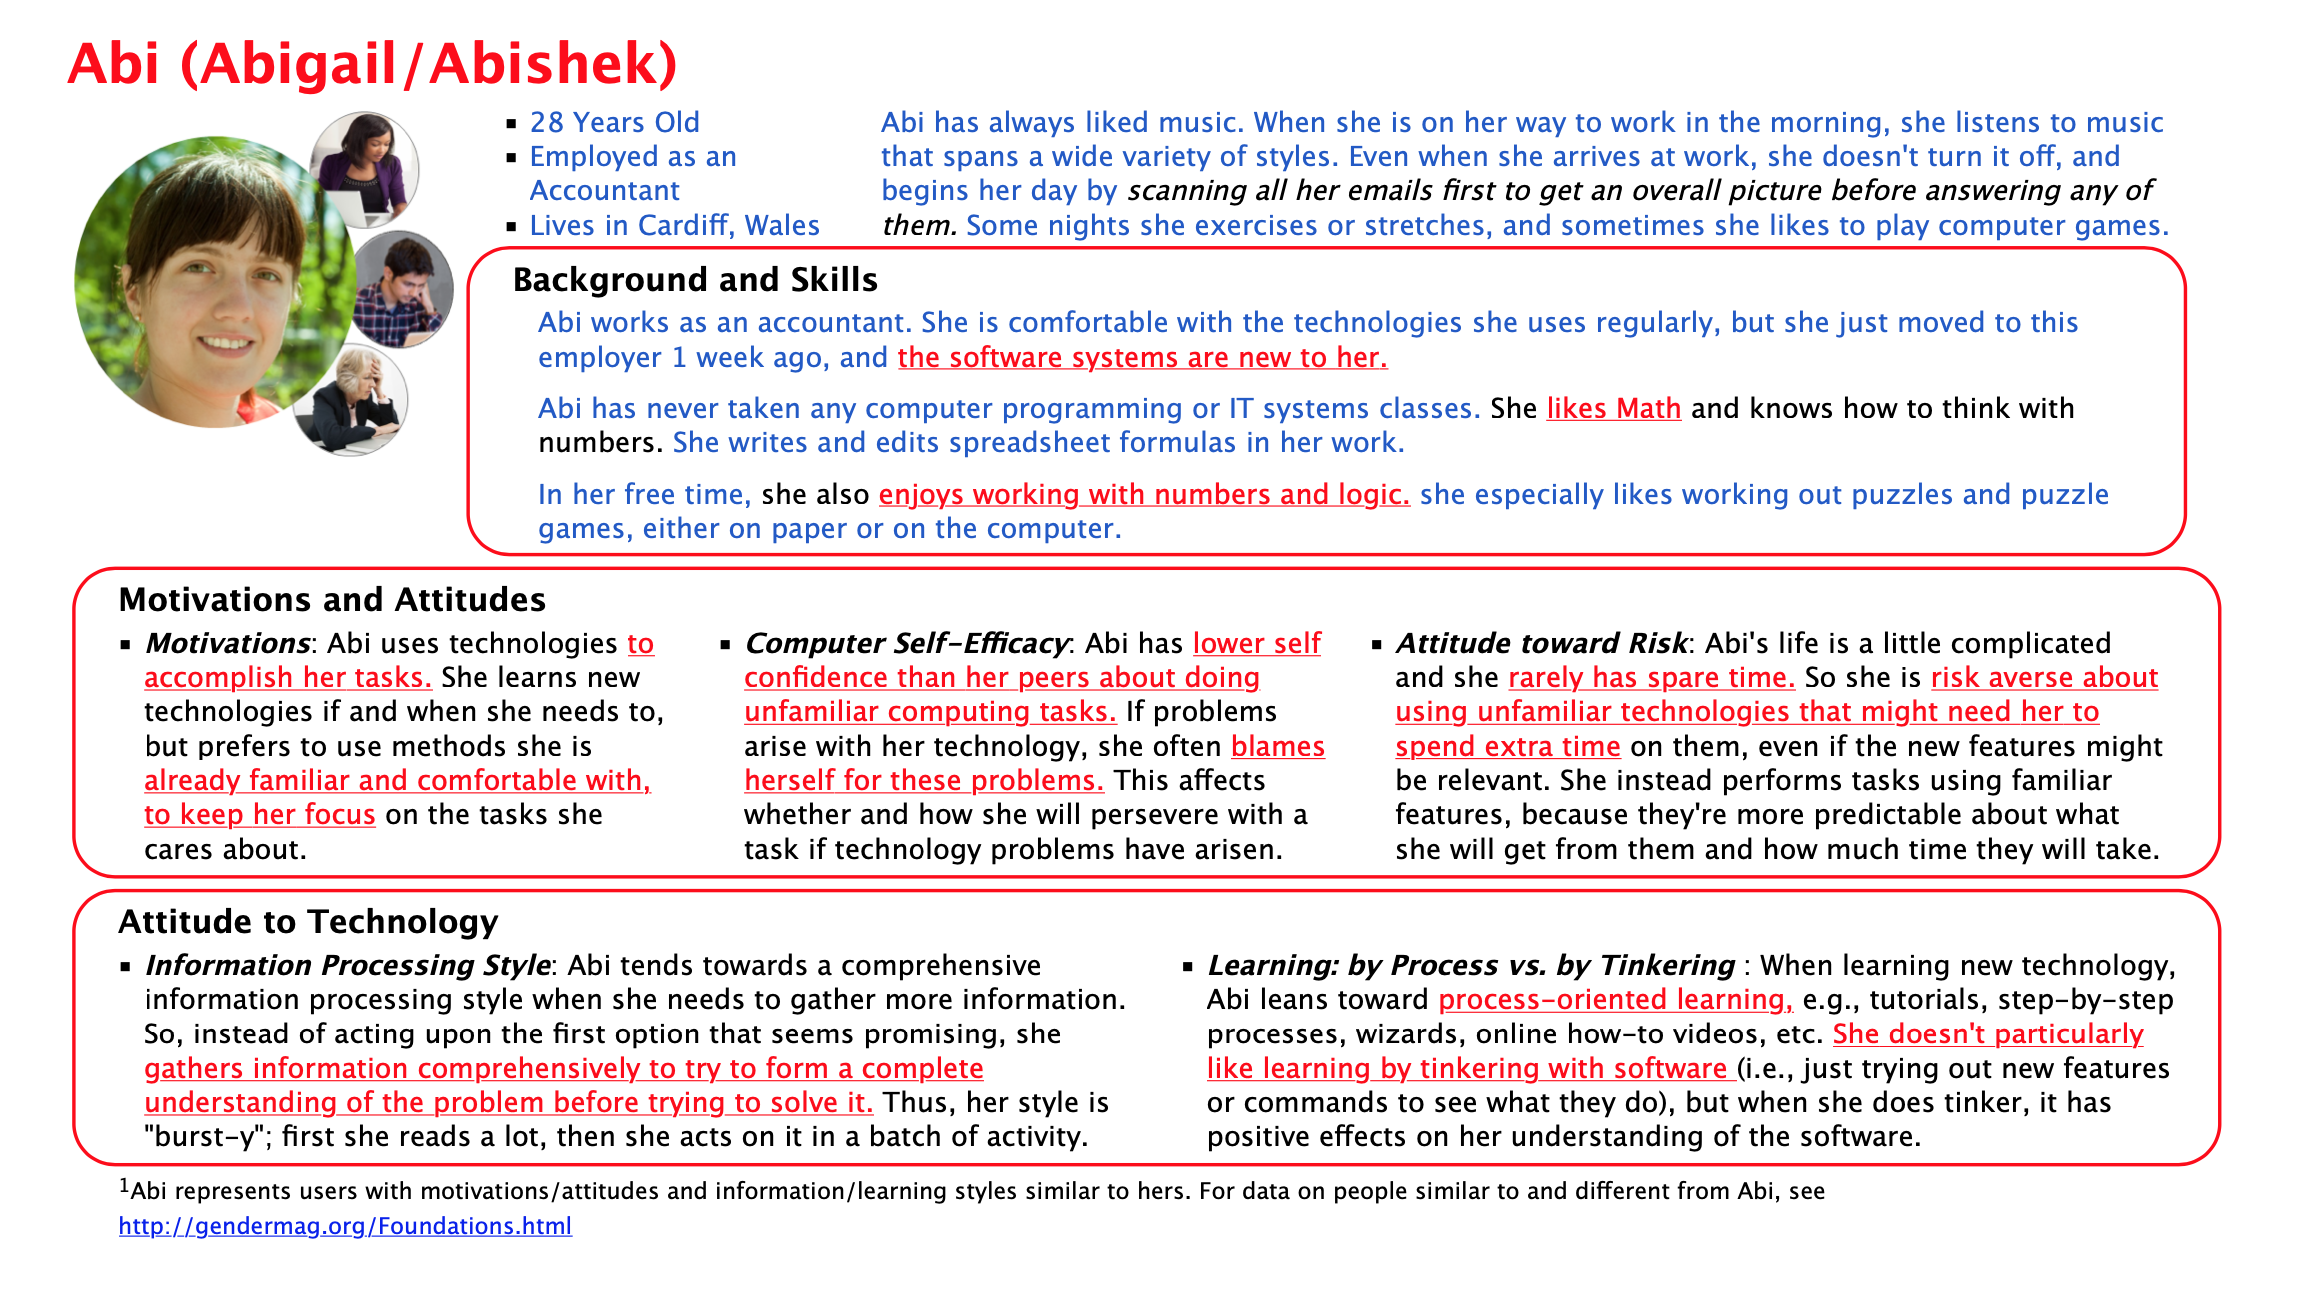
\includegraphics[scale=0.45]{PDFs/Abby.png}
\newpage
\subsection{Walk-through 1}
On the following page the first walk-through will be presented which was made by Mert Erol (20-915-245).
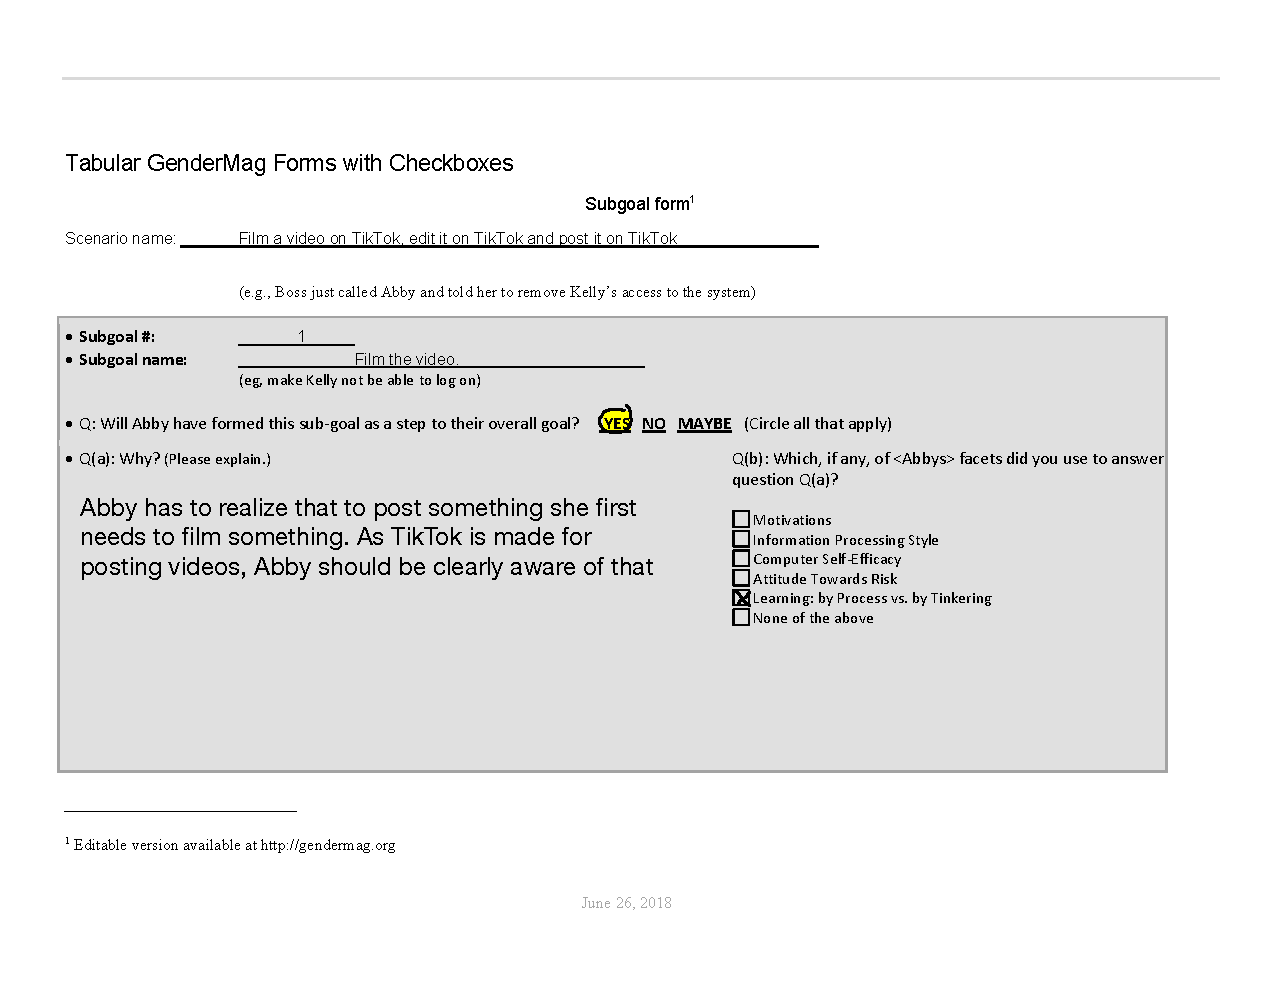
\includepdf[pages=-]{PDFs/Subgoal_Action_1_Mert.pdf}
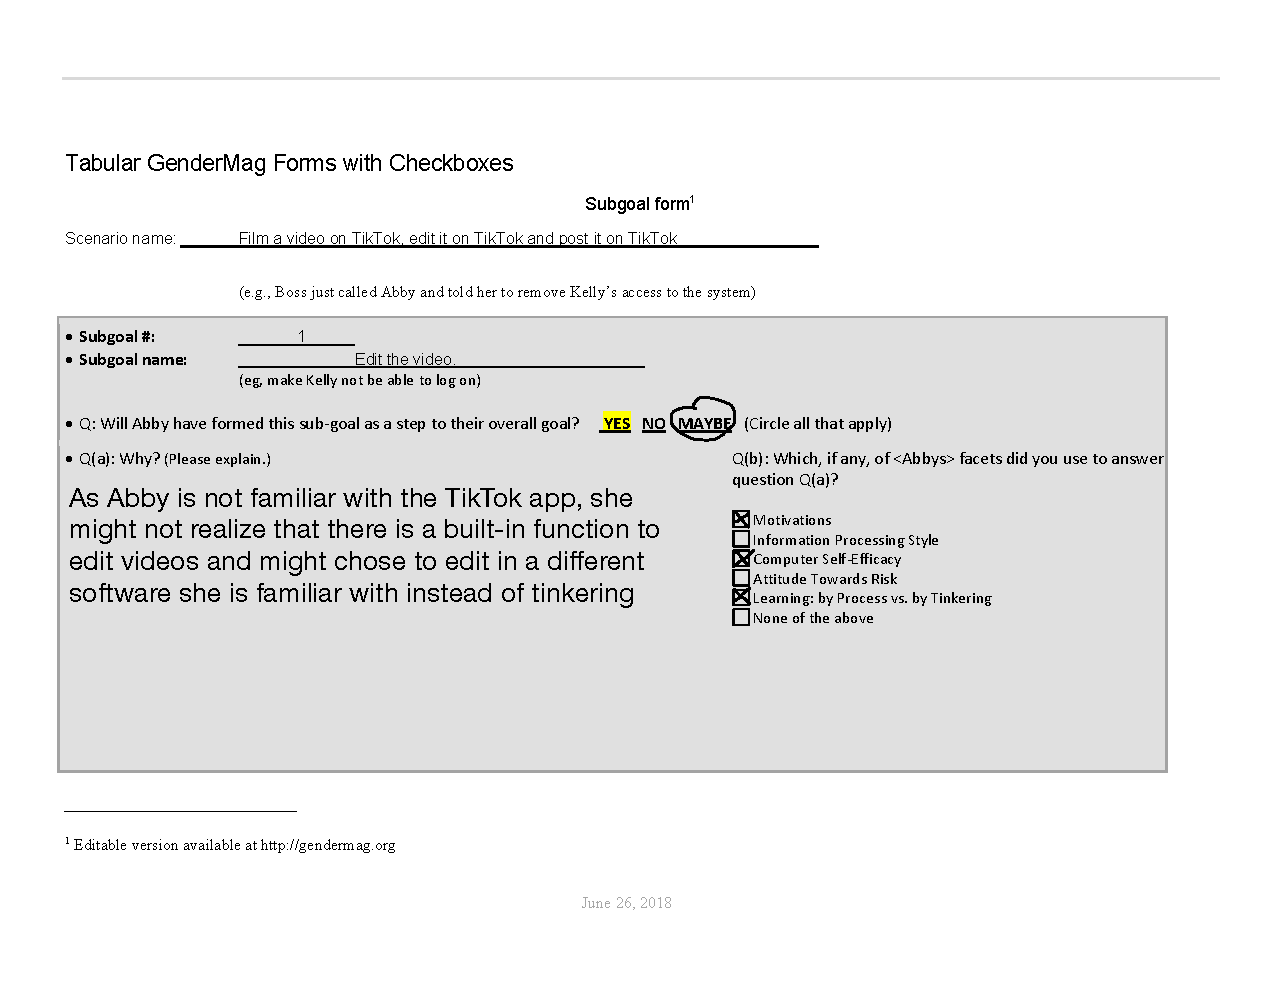
\includepdf[pages=-]{PDFs/Subgoal_Action_2_Mert.pdf}
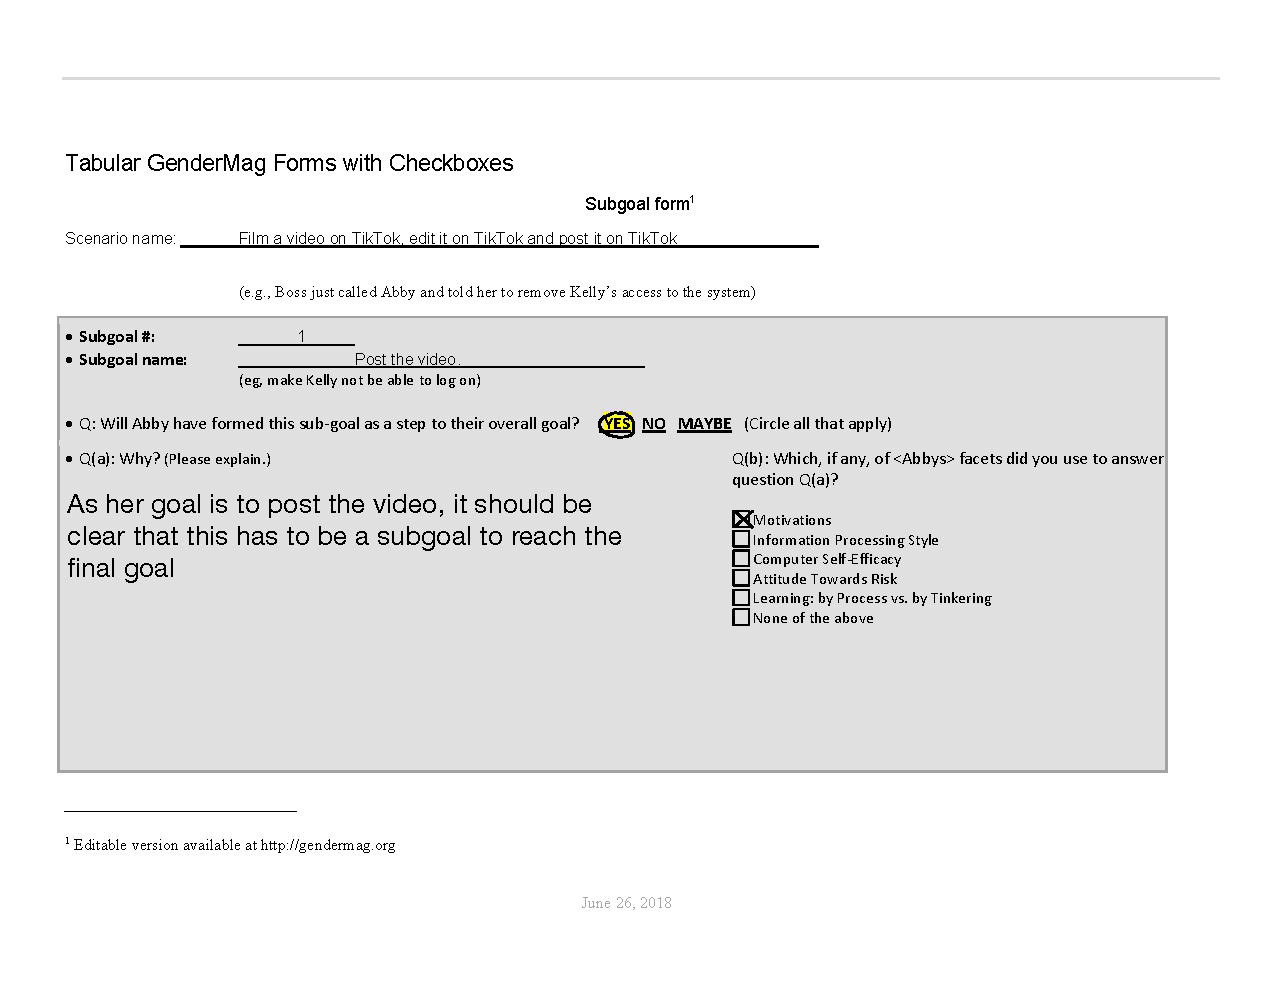
\includepdf[pages=-]{PDFs/Subgoal_Action_3_Mert.pdf}
\subsection{Walk-through 2}
On the following page the first walk-through will be presented which was made by Luc Aggett (20-918-371).
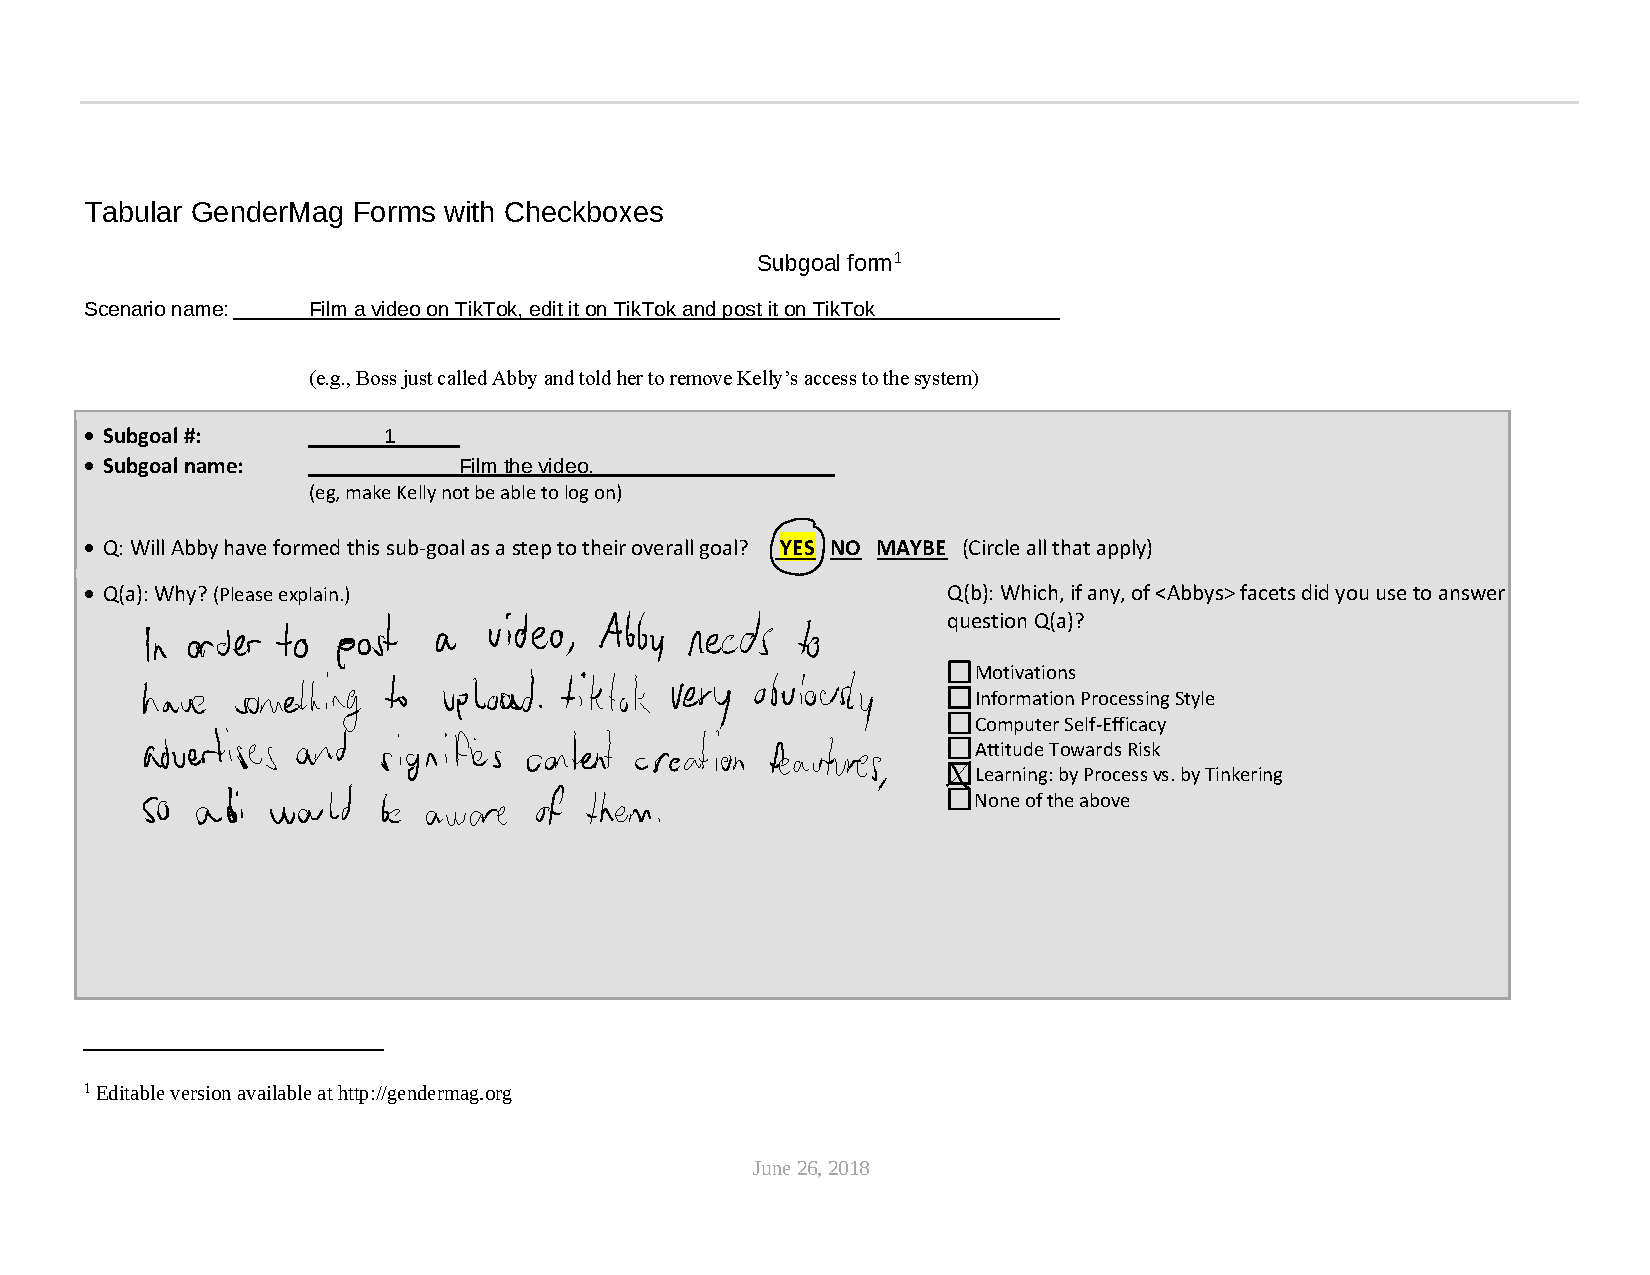
\includepdf[pages=-]{PDFs/Subgoal_Action_1_partner_filled.pdf}
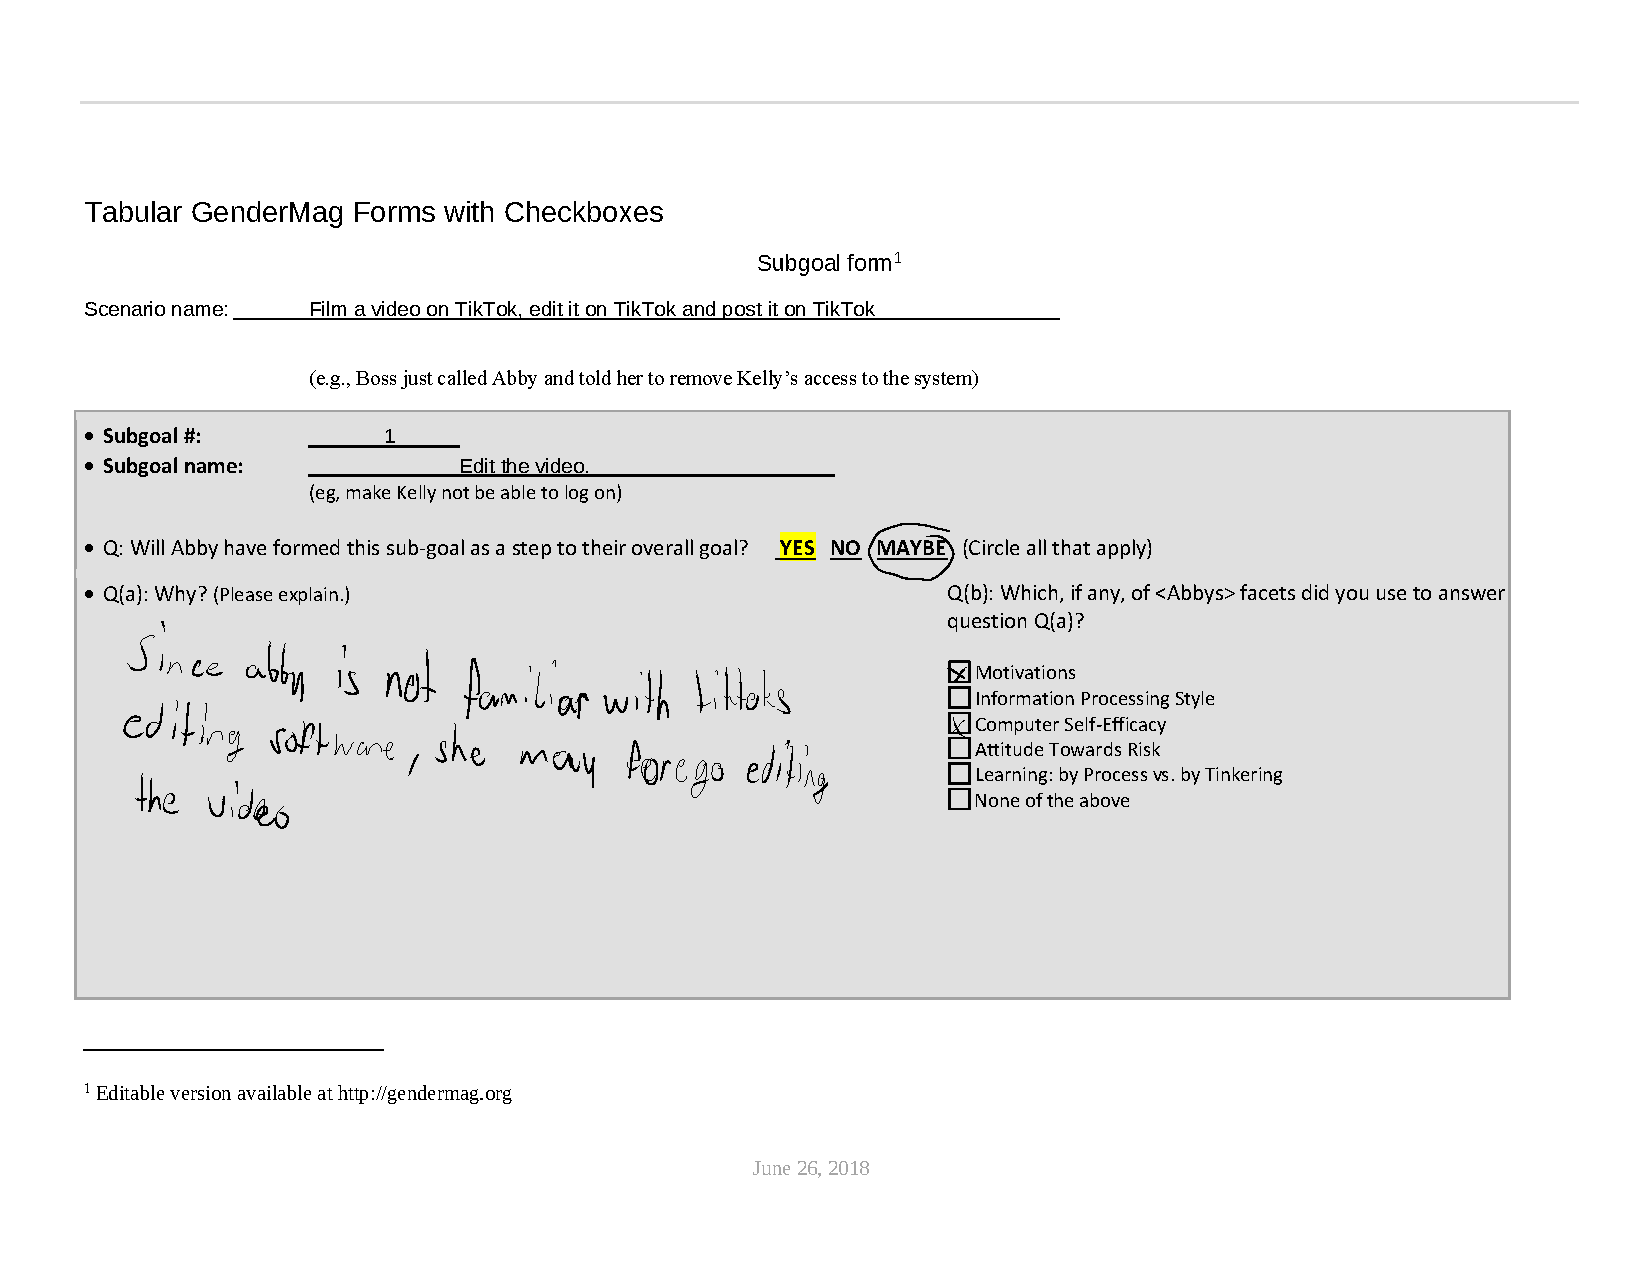
\includepdf[pages=-]{PDFs/Subgoal_Action_2_partner_filled.pdf}
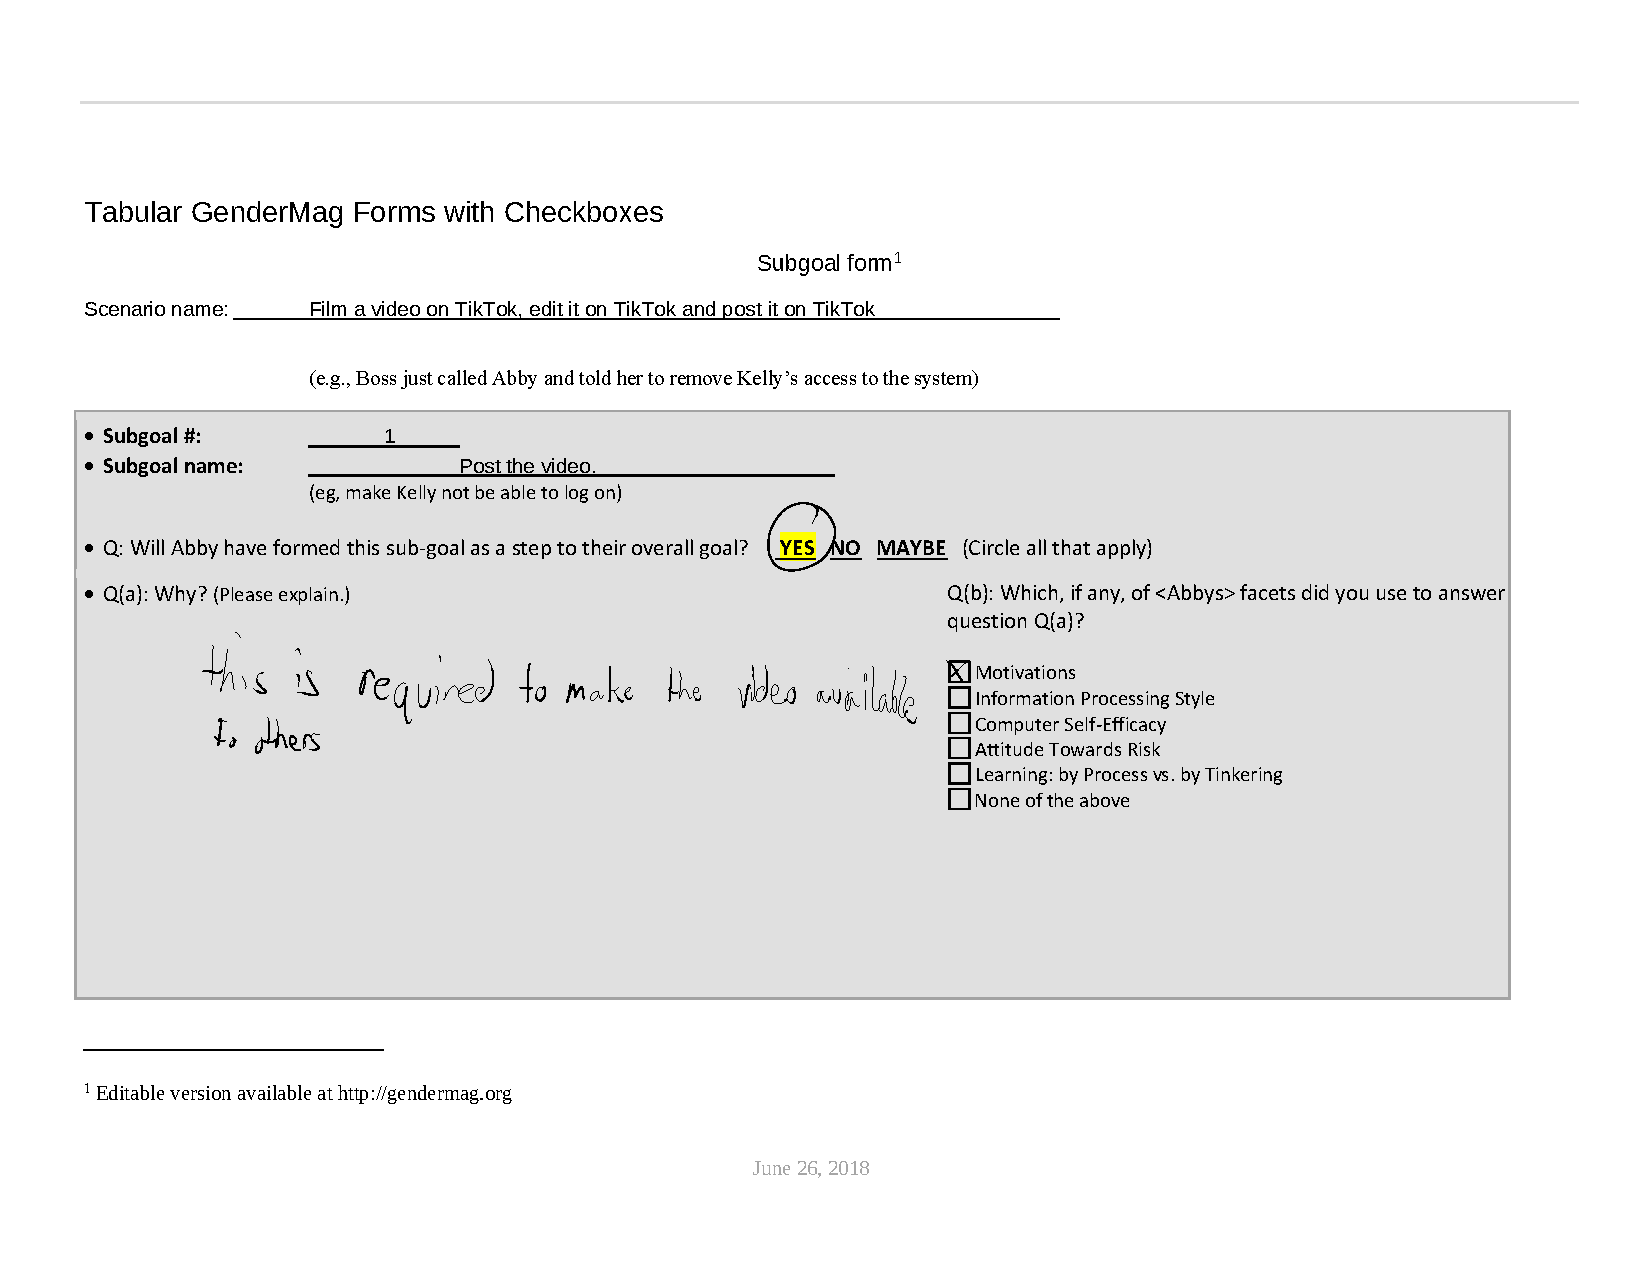
\includepdf[pages=-]{PDFs/Subgoal_Action_3_partner_filled.pdf}

\end{document}
